\documentclass{beamer}

% Setup appearance:

\usetheme{Darmstadt}
\usefonttheme[onlylarge]{structurebold}
\setbeamerfont*{frametitle}{size=\normalsize,series=\bfseries}
\setbeamertemplate{navigation symbols}{}


% Standard packages

\usepackage[brazil]{babel}
\usepackage[latin1]{inputenc}
\usepackage{times}
\usepackage[T1]{fontenc}
\usepackage{amsmath}% http://ctan.org/pkg/amsmath
%\usepackage[table]{xcolor}
\usepackage{multicol}
\usepackage{textcomp} 

% Setup TikZ
\usepackage{tikz}
\usetikzlibrary{arrows}
\tikzstyle{block}=[draw opacity=0.7,line width=1.4cm]

%diretório das figuras
\graphicspath{../article}

\title[Nursery]{%
Nursery%
}

\author[Souza,Medeiros,Santos,Ara�jo]{
     Danilo~Souza\and
     Hugo~Santos\and
     Iago~Medeiros\and
     Welton~Ara�jo
     }


\institute[Bel�m]{
  \inst{1}%
  Universidade Federal do Par�
  }
\date[Bel�m 2012]{
  16 de Julho de 2013
  }



\begin{document}
\section{Bagging usando Prisma e Rede Neural}
\begin{frame}{Testes}
\begin{itemize}
		\item Tamb�m foram realizados testes com bagging em conjunto com o Prisma e Rede Neural.
		\item No caso da Rede Neural foi utilizado o momento = 0.2, taxa de aprendizado = 0.2 e n�mero de ciclos = 100. 
		\item No exemplo utilizando o Weka, ser� variado a quantidade de registros utilizados(porcentagem) e o n�mero de itera��es.
\end{itemize}	
	
\end{frame}

\begin{frame}{Prisma - Variando o n�mero de itera��es}
\begin{figure}
	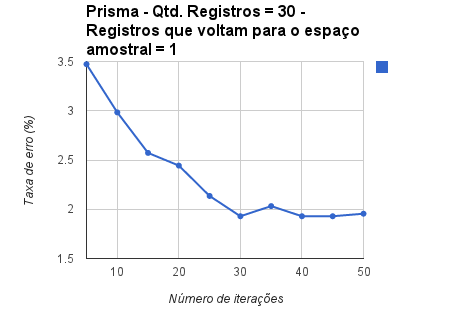
\includegraphics[scale=0.5]{./pictures/Bagging(prisma)QtdReg30Reg1VarNumItXerro.png}
\end{figure}
\begin{itemize}
\item utilizando prisma normal o erro = 1.2088\%
\end{itemize}
\end{frame}

\begin{frame}{Prisma - Variando a quantidade de registros}
\begin{figure}
	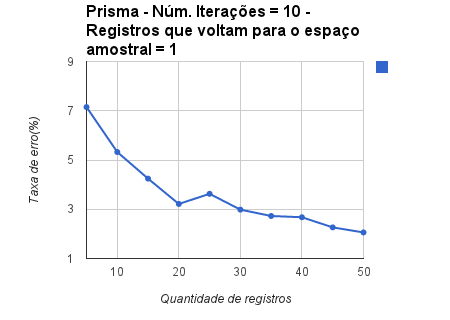
\includegraphics[scale=0.5]{./pictures/Bagging(prisma)NumIt10Reg1VarQtdRegXerro.png}
\end{figure}
\begin{itemize}
\item utilizando prisma normal o erro = 1.2088\%
\end{itemize}
\end{frame}

\begin{frame}{Rede Neural - Variando o n�mero de itera��es}
\begin{figure}
	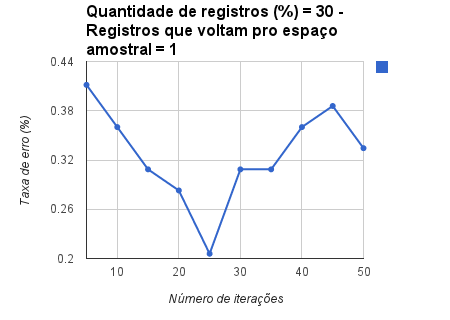
\includegraphics[scale=0.5]{./pictures/Bagging(rede)QtdReg30Reg1VarNumItXerro.png}
\end{figure}
\begin{itemize}
\item utilizando a Rede neural normal o erro = 0.0257%
\end{itemize}
\end{frame}


\begin{frame}{Rede Neural - Variando a quantidade de registros}
\begin{figure}
	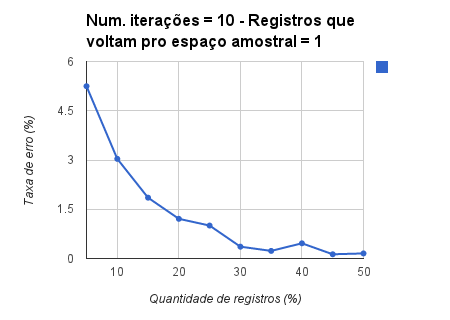
\includegraphics[scale=0.5]{./pictures/Bagging(rede)NumIt10Reg1VarQtdRegXerro.png}
\end{figure}
\begin{itemize}
\item utilizando a Rede neural normal o erro = 0.0257%
\end{itemize}
\end{frame}


\begin{frame}{Conclus�es}
\begin{itemize}
\item Para uma base de dados pequena a mistura com o bagging n�o foi satisfat�ria.
\item N�o foi encontrada implementa��es que realizem a mistura entre os algoritmos como o Random Forest.
\end{itemize}
\end{frame}

\end{document}